\section{Bilag}


\subsection{Mail fra lampedesigner Erik}
\label{sec:mailErik}
Kære Mathias

Det er en meget komplex opgave i der er igang med, der er mange faktorer i spil når det handler om lys, både de fysiske, men ikke mindst de mentale. Jeg har i en del år arbejdet med lampedesign. og har derfor mest været optaget af armaturets/lampens skulpturelle udtryk, men da det jo er en lampe skal den selvfølgelig  også opfylde det belysningsmæssige behov. Jeg har arbejdet med mange lyskilder, lige fra glødepæren til det nyeste LED.I alle mine lamper er valg af lyskilde og placering sket på grundlag af test via prototyper. de fleste af mine lamper er prototyper. En af de mest krævende lamper, har været Gedserlampen, der har et specielt designet armatur, der kan sammensættes til forskellige højder. Gedserlampen er en reflektorlampe, og lyskilden er LED. det krævede utallige målinger, og det foregik såmænd kl 12 om natten, en tommestok på jorden og et luxmeter. Jeg vil nok foretrække prototype test, da de jo er tæt på virkeligheden, men måske kunne jeres software være en god hjælp i den indledende fase af et projekt? Du er velkommen til at kontakte mig igen hvis du tror jeg kan bidrage med noget.

Held og Lykke med projektet.

Venlig hilsen

Erik Mortensen

\subsection{Mail fra lampedesigner David fra IKEA Sverige}
\label{sec:mailDavid}
Hi! Apart from hand sketching and physical prototypes, we use the 3D modeling application Solid Works in IKEA of Sweden. And for renderings we use either the built in renderer, or photo works, which is also part of solid works.

Regards 

//David 

  On 9 October 2015 15:19:41 +08:00, Lasse Fribo Gadegaard <lgadeg15@student.aau.dk> wrote:
   
  Hello
   
   
  We are seven students from Aalborg university, that are writing a project on lamps and how they are design. And so we would like to ask you if you use any software to visualize your design, before they are made as a prototype or finished product. If you use any software feel free to tell us so we could research the software and get a better insight in the industry. I really hope you can help us. Thanks
   
   
  Regards,
  7 Students from Aalborg university
  
\subsection{Mail fra belysningskonsulent}
\label{sec:mailbelysning}

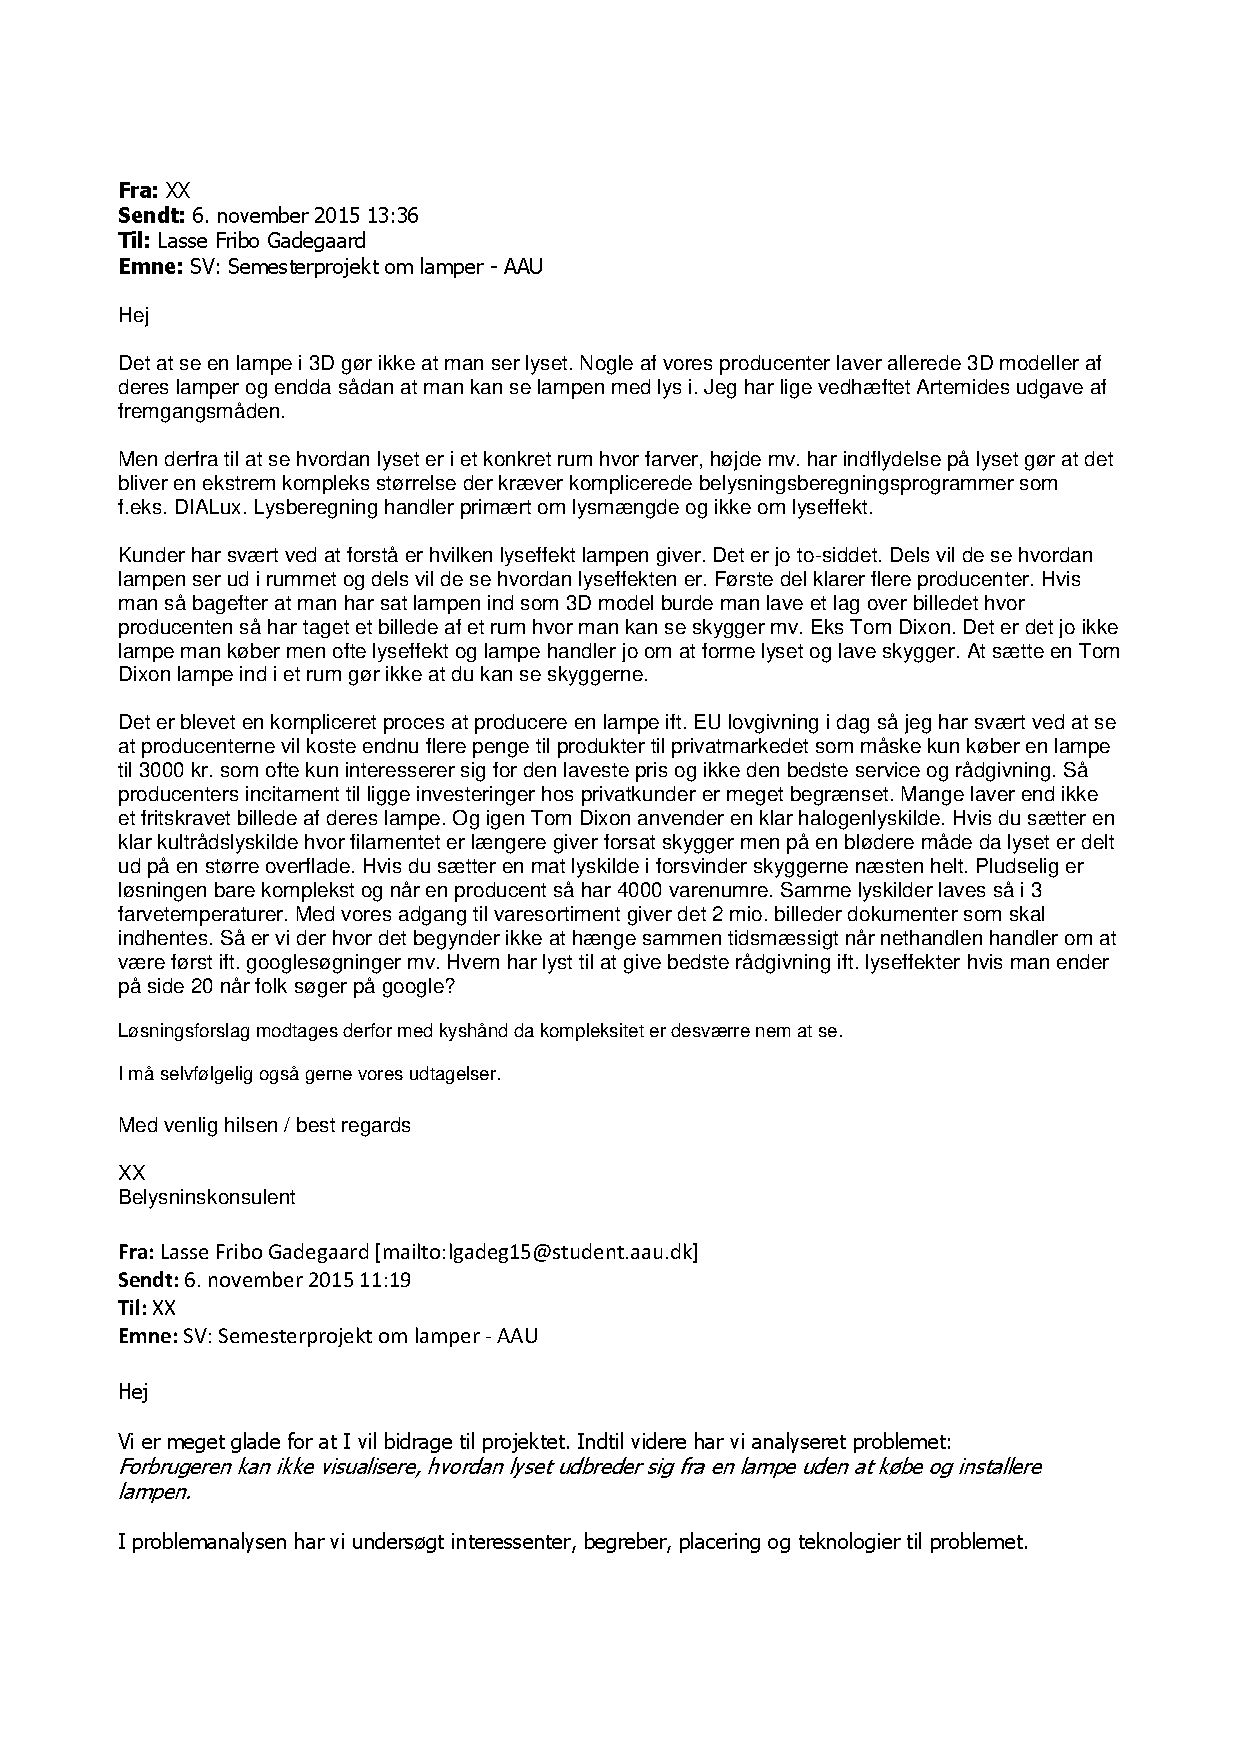
\includepdf[pages={1-3}]{../graphics/mails.pdf}